\section{Síntese de controle PID}
\label{sec:pid}
 
\begin {enumerate}
  \item Antes de definirmos os operadores de mutação e \textit{crossover}, é
  necessário diferenciarmos estes dois conceitos. Embora ambos ocorram em
  organismos biológicos e sejam responsáveis pela alteração do genótipo de um
  indivíduo, estes mecanismos ocorrem em diferentes etapas da vida do respectivo
  organismo. O termo \textit{mutação} é utilizado para descrever o processo no
  qual um alelo de um gene é \textbf{aleatoriamente} substituído ou modificado
  por outro. Em termos matemáticos, sejam os índices \(r, \ldots, u\) as
  posições que sofrerão mutação e que foram determinadas aleatoriamente. Cada
  posição possui um probabalidade \(p_m\) de ser submetida a este processo. Ao
  final da mutação, os alelos referentes a estes índices serão modificados, no
  caso de uma codificação em ponto flutuante, segundo uma distribuição
  \textit{uniforme} ou \textit{não uniforme}. No caso da \textit{não uniforme},
  insere-se uma perturbação com distribuição \textit{normal} com média nula na
  posição escolhida e desvio-padrão decrescente ao longo das gerações, o que
  garante consequentemente um refinamento da solução à medida que nos
  aproximamos de resultados ótimos. 
  
  O processo de \textit{crossover}, por sua vez, trata-se de um mecanismo de
  recombinação genética de dois ou mais cromossomos. Para a codificação de
  algoritmos evolutivos em que os cromossomos possuem valores em ponto
  flutuante, destacam-se duas técnicas: o \textit{crossover} aritmético e o
  uniforme. Para o primeiro, a partir dos cromossomos \(\textbf{x}\) e \(\textbf{y}\),
  obtém-se uma combinção convexa dos valores dos genes de \(\textbf{x}\) e
  \(\textbf{y}\), isto é, o cromossomo \(a\textbf{x} + (1-a)\textbf{y}\), em que
  \(a \in [0, +1]\). Para o segundo, os genes dos cromossomos pais são
  escolhidos com igual probabilidade para formar um cromossomo filho. Por
  exemplo, se a probabilidade vale 0.5, então espera-se que o cromossomo
  resultante seja composto por metade dos genes de \textbf{x} e metade de
  \textbf{y}.
  
  Outra etapa importante para os algoritmos evolutivos é a seleção dos
  indivíduos mais ``adaptados'' ao problema (que possuem maior função de
  \textit{fitness}). Este processo deve garantir que os melhores indivíduos
  persistam, mas não deve ser extremamente radical a fim de garantir uma
  diversidade na população. Um exemplo de um operador de seleção é a técnica de
  \textit{seleção por torneio}. Para selecionar \(N\) indivíduos, realizam-se
  \(N\) torneios com \(p\) participantes, escolhidos aleatoriamente. Quanto mais
  alto é \(p\), maior é a pressão seletiva, isto é, para um indivíduo ruim ser
  escolhido ao menos em um torneio, é necessário que ele compita com \(p-1\)
  indivíduos piores que ele (para \(p\) grande, a probabilidade deste fato
  ocorrer é muito pequena). Cada torneio é vencido pelo indivíduo que apresenta maior
  \textit{fitness}. No caso deste exercício, será realizado apenas um torneio,
  que é composto por 3 indivíduos.

  \item As constantes rrier 
    apresentadas na tabela \ref{tab:pid_constantes} a seguir
  foram definidas no arquivo \texttt{prog\_PID.m}, disponibilizado pelo
  professor.
  
  \begin{table}[h]
	    \centering
		\caption{\label{tab:pid_constantes} Constantes definidas em
		\texttt{prog\_PID.m}}
		\begin{tabular}{|c | c |}
			\hline
			\textbf{Atributos} & \textbf{Valor} \\	\hhline{|=|=|}
			Tamanho da População & 100 \\ \hline 
			Número máximo de Gerações & 50 \\ \hline 
			Taxa de Mutação & 0.4 \\ \hline 			
			Taxa de Crossover & 0.8 \\ \hline 			
		\end{tabular}	    
    \end{table} 
    
    Observa-se taxas de mutação e \textit{crossover} relativamente altas: para a
    primeira, um alelo tem probalidade de 40\% de ser mutado, isto é, ele possui
    aproximadamente a metade das chances de ser modificado. Em relação ao
    tamanho da população e o número de gerações , 100 e 50 são
    números suficientemente grandes para garantir, respectivamente,	 diversidade
    entre os indivíduos e uma boa qualidade no resultado visto a quantidade de
    recombinações entre os cromossomos que serão realizadas.
    
    A população inicial é obtida pelo comando \texttt{pop =
    5*rand(tam\_pop,3);}, em que \texttt{rand} é uma função do MATLAB que gera
    números aleatórios segundo uma distribuição uniforme e \texttt{tam\_pop}
    vale 100. Será criada, portanto, uma matriz de 100 linhas, cada uma
    representando um indivíduo, e 3 colunas, uma para cada constante a ser
    determinada \(k_p\), \(k_d\) e \(k_i\).
    
    Finalmente, cada operador de \textit{crossover} é escolhido com 50\% de
    probabilidade. Espera-se portanto que o operador aritmétido seja escolhido
    em metade das oportunidades e o uniforme, também.
    
    \item Após adicionarmos as linhas referentes ao cálculo do \textit{fitness},
    as execuções do programa \textit{prog\_pid.m} resultam nos dados da tabela
    \ref{tab:pid_c}.
    
    \begin{table}[h]
	    \centering
		\caption{\label{tab:pid_c} Resultados das 5 execuções de
		\texttt{prog\_PID.m}}
		\begin{tabular}{| c | c | c | c | c | c | c | c | c |}
			\hline
			\textbf{Ex.} & \(k_p\) & \(k_d\) & \(k_i\) &
			\(t_{subida} \) (s) & \(t_{estabilizacao}\) (s) & \textit{Overshoot} (\%) &
			\(\Delta \phi\) (º)& \textit{Fitness}\\ \hhline{|=|=|=|=|=|=|=|=|=|}
			1 & 4.9935 & 2.385e-05 & 4.46633 & 0.0064396 & 3.26286 &  97.7286  &
			1.1935 & 9.9360\\ \hline 
			2 & 4.9960 & 2.296e-05 & 3.99303 & 0.0064393 & 3.14669 & 97.6506 & 
			1.2340 & 9.9360 \\
			\hline 3 & 4.9923 & 1.350e-05 & 3.95399 & 0.0064397 & 3.3217 & 97.7735 &
			1.1687 & 9.9360	\\
			\hline 4 & 4.9940 & 2.240e-05 & 4.33452 & 0.0064395 & 3.24405 & 97.7234 &
			1.1960 & 9.9360\\
			\hline 5 & 4.9990 & 1.528e-05 & 4.4244 & 0.0064348 & 3.41617  & 97.8392 &
			1.1346 & 9.9361 \\ 
			\hline
		\end{tabular}	    
    \end{table}
    
    Observa-se que todos os valores \(k_d\) relativos à ação derivadora são
    praticamente nulos e que \(k_i\) e \(k_p\) encontram-se muito próximos a
    seus valores máximos, isto é, 5. Isto indica que a ação derivadora não
    exerce efeitos importantes sobre o tempo de resposta apresentado pelo
    sistema.    Os valores de tempo dos primeiros máximos em todas as execuções
    concentram-se em torno do valor \(t_{subida} = 0.00644\) s. Sabe-se também
    que este atributo é fortemente ligado à frequência de oscilação que a
    resposta ao degrau apresentará. Para sistemas de segunda ordem, por exemplo,
    a relação \(w_0t_m \approx 3\) evidencia o compromisso entre essas duas
    características.  Portanto, para valores muito pequenos de \(t_{subida}\),
    teremos frequências \(w_0\) elevadas e vice-versa. É justamente esse
    comportamento que é observado neste caso: pelo fato de que a função de
    \textit{fitness} só levar em conta o tempo de resposta, obtém-se respostas
    muito rápidas, porém que oscilam fortemente em torno de 1. A margem de fase
    (\(\Delta \phi\)) também possui uma relação com o \textit{overshoot}:
    pequenas margens de fase produzem sistemas menos estáveis e que apresentam
    maior erros percentuais entre a entrada e a saída. No nosso caso, como não
    nos preocupamos com esse parâmetro, obtém-se pequenas margens de fase e,
    consequentemente, grandes erros antes da estabilização. A figura
    \ref{fig:pid_step_c}, que é o resultado de uma das execuções acima, permite
    a visualização destes comportamentos. A figura \ref{fig:pid_mutacao_c}, por
    sua vez, mostra a quantidade de mutações realizadas pelo algoritmo evolutivo
    no decorrer no programa. Conforme explicado anteriormente, essa quantidade
    deve ser decrescente, visto que os melhores indíviduos devem ser mantidos
    nas gerações finais. As figuras \ref{fig:pid_fitness_c} e
    \ref{fig:pid_parametros_c} mostram, respectivamente, a evolução dos valores
    da função de \textit{fitness} e dos parâmetros \(k_p\), \(k_i\) e \(k_d\).
    Para o primeiro, observa-se que o melhor \textit{fitness} permanece sempre
    próximo de 10 e que o \textit{fitness} médio aproxima-se gradualmente a este
    valor, indicando que a população esta se ``especializando'' e adaptando no
    problema. Para segundo, verifica-se que \(k_d\) é praticamente nulo em todas
    as gerações, \(k_p\) se estabiliza a partir da geração 10 e \(k_i\) varia
    fortemente até a geração 40. Estes fatos nos dizem que o parâmetro que mais
    influencia o tempo do primeiro máximo é a ação integradora.

    \FloatBarrier
			    
	\begin{figure}[h!]
	
	\centering
	
		\begin{subfigure}{.5\textwidth}
		  \centering
		  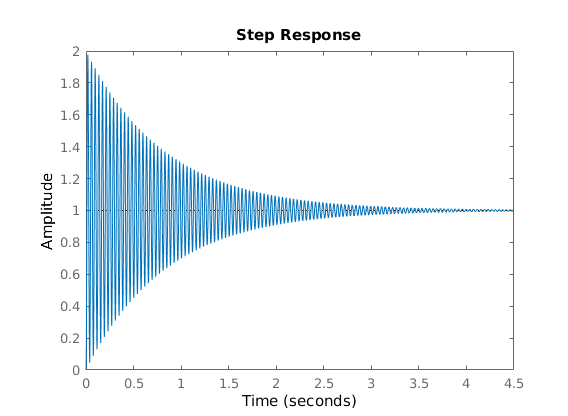
\includegraphics[width=1\linewidth]{image/step_pid_ex_c}
		  \caption{Resposta ao degrau do sistema.}
		  \label{fig:pid_step_c}
		\end{subfigure}%
		\begin{subfigure}{.5\textwidth}
		  \centering
		  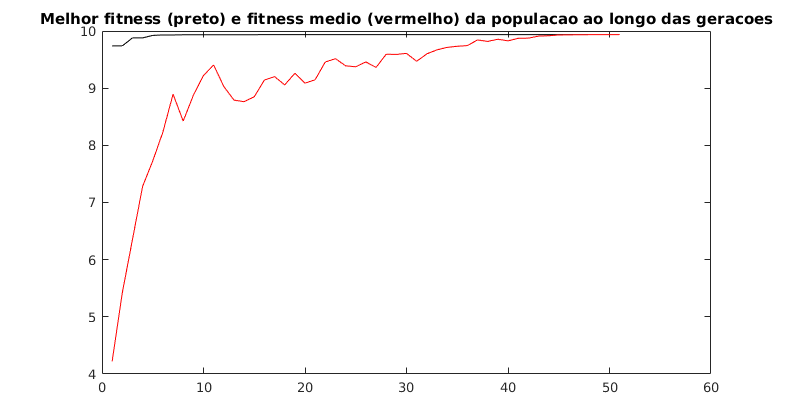
\includegraphics[width=1\linewidth]{image/melhor_fitness_pid_ex_c}
		  \caption{Evolução dos valores da função \textit{fitness}.}
		  \label{fig:pid_fitness_c}
		\end{subfigure}%
		
		\begin{subfigure}{.5\textwidth}
		  \centering
		  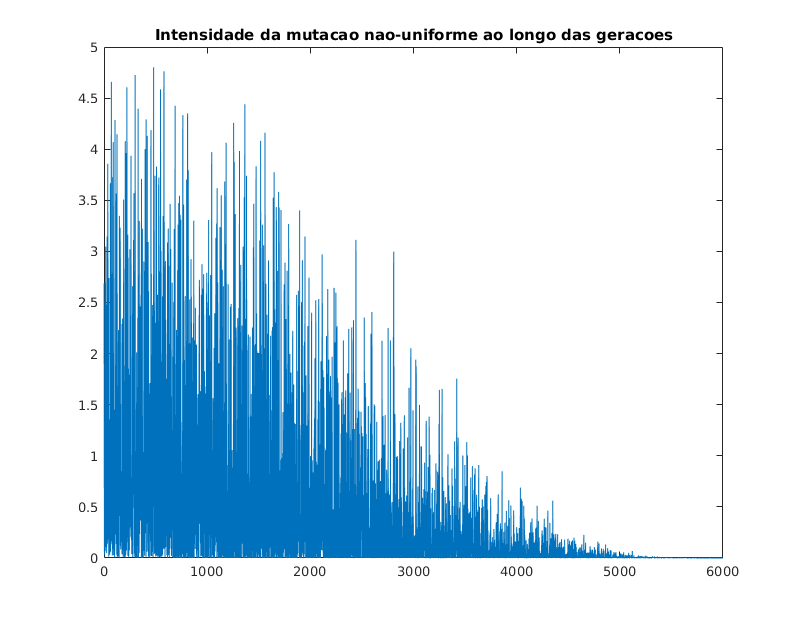
\includegraphics[width=1\linewidth]{image/mutacao_pid_ex_c}
		  \caption{\centering Evolução da intensidade de mutações ao longo das
		  gerações.}
		  \label{fig:pid_mutacao_c}
		\end{subfigure}%
		\begin{subfigure}{.5\textwidth}
		  \centering
		  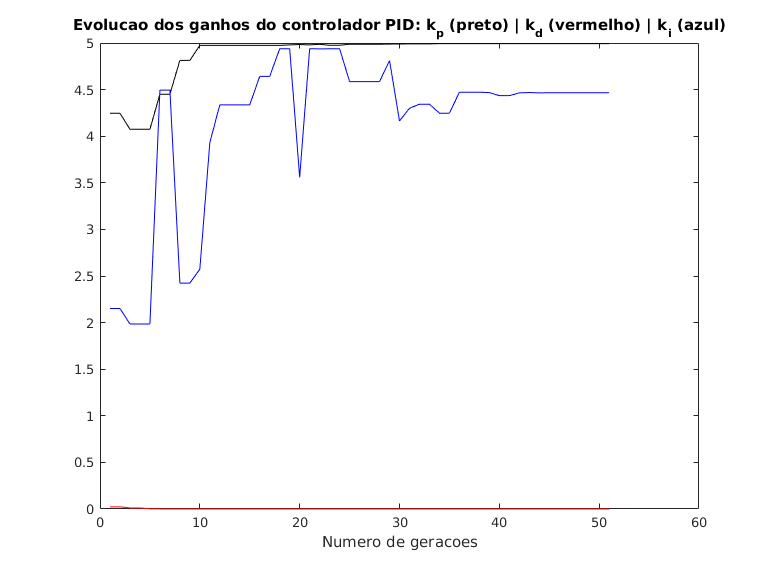
\includegraphics[width=1\linewidth]{image/kp_kd_ki_pid_ex_c}
		  \caption{\centering Evolução dos parâmetros.}
		  \label{fig:pid_parametros_c} 
		\end{subfigure}
	
	\caption{Resultado para a execução 1 do algoritmo evolutivo.}
	\end{figure}
	
	
	\FloatBarrier
	
	 A modificação dos parâmetros da tabela \ref{tab:pid_constantes} pode
	 influenciar nos resultados acima. Se dobrarmos o número de indivíduos na
	 população, isto é, 200, e aumentarmos as taxas de crossover e mutação para,
	 respectivamente, 0.9 e 0.6, obtém-se os dados contidos na tabela
	 \ref{tab:pid_c_2}.
    
    \begin{table}[h]
	    \centering
		\caption{\label{tab:pid_c_2} Resultados da execução com os parâmetros
		modificados.}
		\begin{tabular}{| c | c | c | c | c | c | c | c |}
			\hline
			\(k_p\) & \(k_d\) & \(k_i\) &
			\(t_{subida} \) (s) & \(t_{estabilizacao}\) (s) & \textit{Overshoot} (\%) &
			\(\Delta \phi\) (º)& \textit{Fitness}\\ \hhline{|=|=|=|=|=|=|=|=|}
			4.9975 & 7.80994e-06 & 4.6839 & 0.00643281 & 3.68641 &  97.9919  &
			1.05405 & 9.93608\\ \hline 
		\end{tabular}	    
    \end{table}
    
    Observa-se que o tempo do primeiro máximo é ligeiramente inferior aos dos
    casos anteriores e, consequentemente, a função de \textit{fitness} é
    superior.  Os valores dos parâmetros continuam parecidos, sendo que \(k_d\)
    é inferior e \(k_i\) superior. De maneira geral, o aumento de recursos
    computacionais disponibilizados ao programa (aumento de população e
    quantidade de mutações) não causaram grandes diferenças nos resultados. As
    figuras \ref{fig:pid_fitness_c_mod} e \ref{fig:pid_parametros_c_mod}
    apresentam o mesmo comportamento descrito no parágrafo anterior e a
    \ref{fig:pid_mutacao_c_mod} destaca que a quantidade de mutações realizadas
    foi muito superior aos casos anteriores: observa-se que a presença de
    quantidades superiores a 10000 quando a taxa de mutação é 0.6.

	\FloatBarrier
			    
	\begin{figure}[h!]
	
	\centering
	
		\begin{subfigure}{.5\textwidth}
		  \centering
		  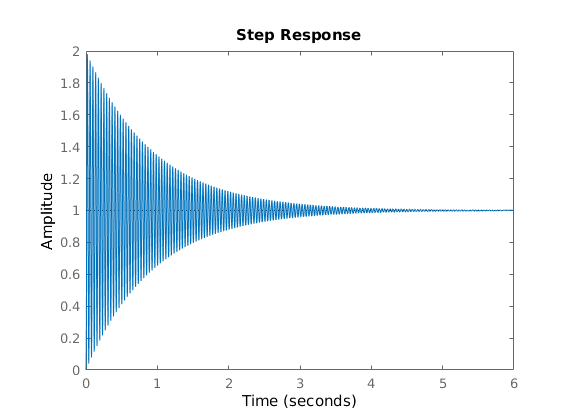
\includegraphics[width=1\linewidth]{image/step_pid_ex_c_mod}
		  \caption{Resposta ao degrau do sistema.}
		  \label{fig:pid_step_c_mod}
		\end{subfigure}%
		\begin{subfigure}{.5\textwidth}
		  \centering
		  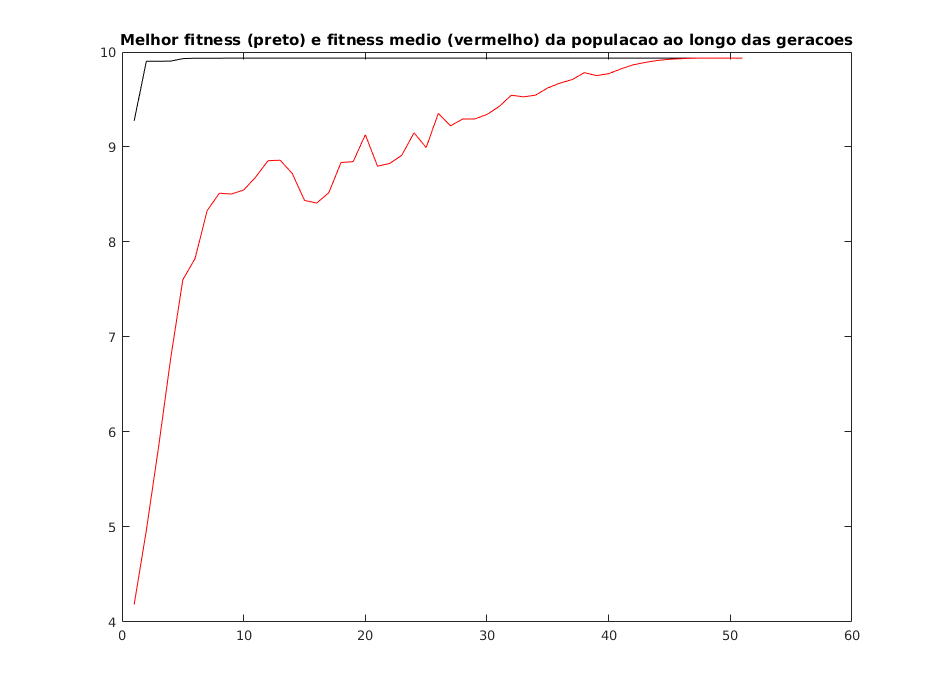
\includegraphics[width=1\linewidth]{image/melhor_fitness_pid_ex_c_mod}
		  \caption{Evolução dos valores da função \textit{fitness}.}
		  \label{fig:pid_fitness_c_mod}
		\end{subfigure}%
		
		\begin{subfigure}{.5\textwidth}
		  \centering
		  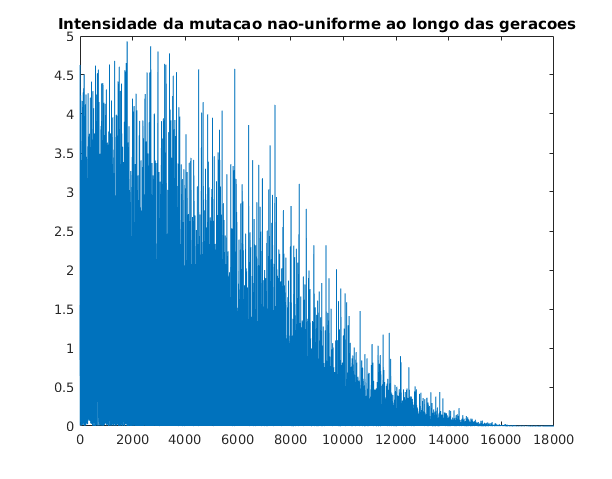
\includegraphics[width=1\linewidth]{image/mutacao_pid_ex_c_mod}
		  \caption{\centering Evolução da intensidade de mutações ao longo das
		  gerações.}
		  \label{fig:pid_mutacao_c_mod}
		\end{subfigure}%
		\begin{subfigure}{.5\textwidth}
		  \centering
		  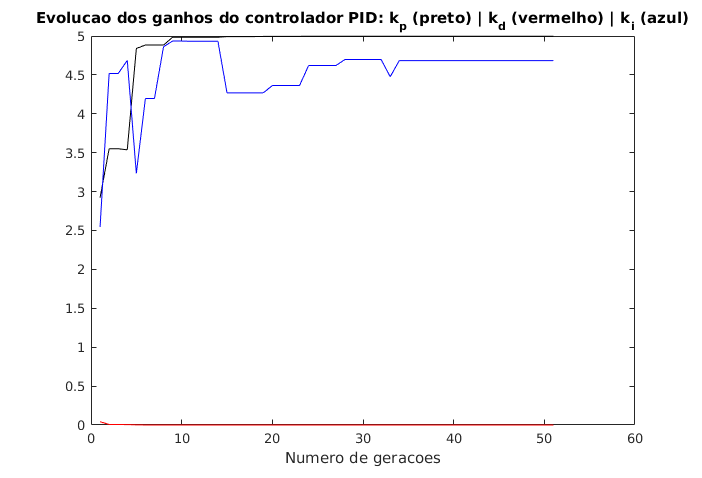
\includegraphics[width=1\linewidth]{image/kp_kd_ki_pid_ex_c_mod}
		  \caption{\centering Evolução dos parâmetros.}
		  \label{fig:pid_parametros_c_mod} 
		\end{subfigure}
	
	\caption{Resultado para a execução do algoritmo evolutivo com parâmetros
	modificados.}
	\end{figure}

	\FloatBarrier
	
	\item Os resultados das 5 execuções com a nova função de \textit{fitness} estão
	presentes na tabela \ref{tab:pid_d}, logo abaixo. Dessa vez, considera-se
	também a margem de fase.
	
	\FloatBarrier
	
	\begin{table}[h]
	    \centering
		\caption{\label{tab:pid_d} Resultados das 5 execuções de
		\texttt{prog\_PID.m}}
		\vspace{-12pt}	
		\begin{tabular}{| c | c | c | c | c | c | c | c | c |}
			\hline
			\textbf{Ex.} & \(k_p\) & \(k_d\) & \(k_i\) &
			\(t_{subida} \) (s) & \(t_{estabilizacao}\) (s) & \textit{Overshoot} (\%) &
			\(\Delta \phi\) (º)& \textit{Fitness}\\ \hhline{|=|=|=|=|=|=|=|=|=|}
			1 & 1.22881 & 0.718353 & 4.54691 & 0.705398 & 12.7319 &  56.4502  &
			59.9346 & 5.53763\\ \hline 
			2 & 1.15518 & 0.57906 & 4.97227 & 0.605573 & 10.924 & 56.4079  & 
			59.9872 & 5.86308 \\
			\hline 3 & 0.812793 & 0.298811 & 4.76622 & 0.44429  & 8.01846 & 56.4355 &
			59.9522 & 6.47451	\\
			\hline 4 & 1.67979 & 1.23205 & 4.94384 & 0.885861 & 15.9772 & 56.398  &
			56.398  & 5.0356 \\
			\hline 5 & 2.36522 & 0.00523679 & 1.84369 & 0.0124718 & 0.100391 & 30.9773 &
			59.986 & 8.98883 \\ 
			\hline
		\end{tabular}	    
    \end{table}
    
    \FloatBarrier
    
    Ao contrário do item anterior, verifica-se neste caso uma grande variação
    nos melhores resultados nas diferentes execuções. As soluções 1 e 2
    apresentam soluções muito parecidas em todos os aspectos. A solução 4 foi a
    pior a ser encontrada e possui o maior valor de \(k_d\) encontrado. Isso
    leva a crer que grandes valores deste parâmetro influenciam negativamente no
    resultado, principalmente em relação à margem de fase: a pior margem foi
    encontrada nesta execução. A solução 5 foi aquela que melhor encontrou um
    compromisso entre tempo do primeiro máximo e estabilidade e, portanto,
    possui o maior \textit{fitness}. Remarcamos que os tempos de subida e
    estabilização e o \textit{overshoot} desta resposta foram muito inferiores a
    aqueles encontrados nas outras execuções, confirmando ainda mais a qualidade
    desta solução. Novamente, nos deparamos com o fato de que o ajuste de \(k_d\) é o
    mais sensível: grandes valores deste parâmetro não levam a bons resultados.
    Observa-se ainda que os outros dois parâmetros, \(k_p\) e \(k_i\), também
    apresentam grandes variações em relação as outras execuções, sendo \(k_d\)
    muito superior e \(k_i\) inferior. As imagens a seguir contém os gráficos
    gerados para a melhor execução. 
    
    \FloatBarrier
			    
	\begin{figure}[h!]
	
	\centering
	
		\begin{subfigure}{.5\textwidth}
		  \centering
		  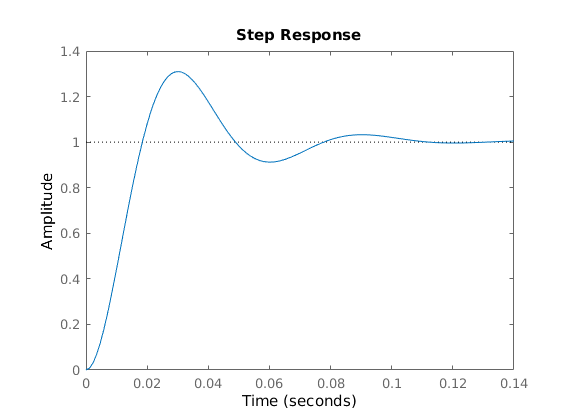
\includegraphics[width=1\linewidth]{image/step_pid_ex_d_5}
		  \caption{Resposta ao degrau do sistema.}
		  \label{fig:pid_step_d_5}
		\end{subfigure}%
		\begin{subfigure}{.5\textwidth}
		  \centering
		  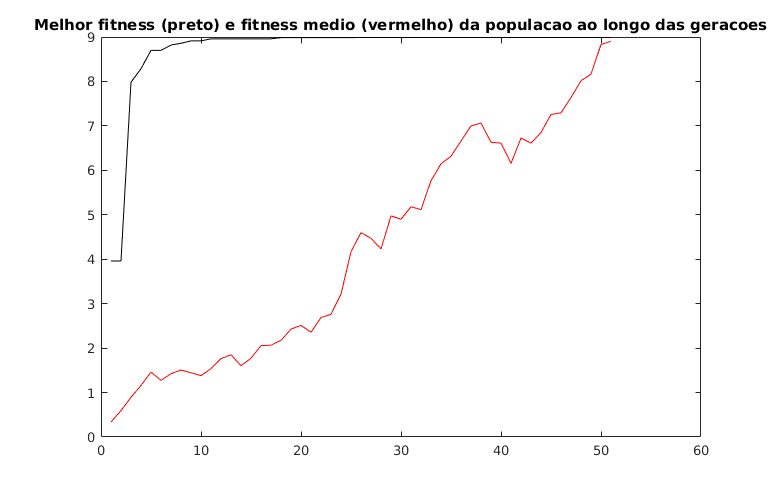
\includegraphics[width=1\linewidth]{image/mutacao_pid_ex_d_5}
		  \caption{Evolução dos valores da função \textit{fitness}.}
		  \label{fig:pid_fitness_d_5}
		\end{subfigure}%
		
		\begin{subfigure}{.5\textwidth}
		  \centering
		  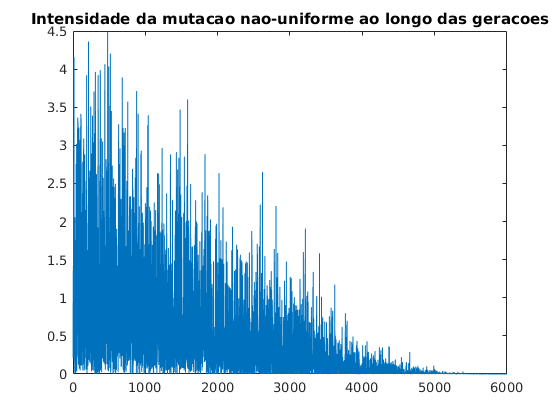
\includegraphics[width=1\linewidth]{image/melhor_fitness_pid_ex_d_5}
		  \caption{\centering Evolução da intensidade de mutações ao longo das
		  gerações.}
		  \label{fig:pid_mutacao_d_5}
		\end{subfigure}%
		\begin{subfigure}{.5\textwidth}
		  \centering
		  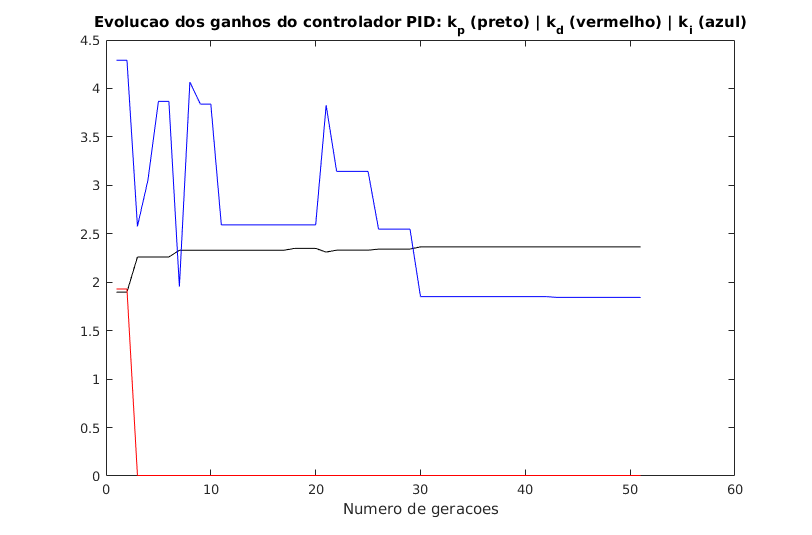
\includegraphics[width=1\linewidth]{image/kp_kd_ki_pid_ex_d_5}
		  \caption{\centering Evolução dos parâmetros.}
		  \label{fig:pid_parametros_d_5} 
		\end{subfigure}
	
	\caption{Resultado para a melhor execução do algoritmo evolutivo com
	\textit{fitness} considerando a margem de fase.}
	\end{figure}
	
	\FloatBarrier
	
	A figura \ref{fig:pid_step_d_5} representa a resposta ao degrau do sistema com
	os parâmetros determinados na execução 5, cujas características já foram
	discutidas no parágrafo anterior. Na imagem \ref{fig:pid_fitness_d_5}, que
	apresenta a evolução do \textit{fitness}, observa-se que o melhor valor já é
	encontrado nas primeiras gerações. Entretanto, a quantia média ainda é muito
	inferior a tal valor, o que implica que a população é muito diversificada até a
	geração 50, isto é, poucos indivíduos se ``adaptaram'' tão bem quanto o
	melhor. A figura \ref{fig:pid_parametros_d_5} revela que o parâmetro que mais
	variou entre as gerações foi \(k_p\), assim como no caso do item anterior.
	
	\vspace{12pt}
	
	Os resultados obtidos com a função \textit{fitness} considerando
	o tempo de subida e também a margem de fase foram muito superiores em muitos
	aspectos:
	
	\begin{itemize}
		\item os valores de \textit{overshoot} no caso anterior eram, em média,
		de 97\%, sendo que neste item, encontra-se 30\%;
		
		\item a margem de fase no item anterior (\(\approx 2º\)) era muito inferior ao
		caso atual, em que exige-se \(\Delta \phi = 60º\), comprometendo fortemente a
		estabilidade do sistema;
	
		\item o tempo de subida no caso anterior era muito inferior ao atual, porém sua
		frequência de oscilação em torno de 1 era inaceitável;
	 
		\item no caso anterior, a resposta demorava muito a se estabilizar, o que pode
		representar um problema para algumas aplicações. No caso atual, encontra-se
		tempos de estabilização na ordem de centésimos de segundo;
	
	\end{itemize} 
	
	Enfim, efetuando as mesmas modificações realizadas anteriormente no tamanho da
	população e nas taxas de crossover e mutação, encontra-se os dados da tabela
	\ref{tab:pid_d_mod} e a imagems a seguir:
	
	\begin{table}[h]
	    \centering
		\caption{\label{tab:pid_d_mod} Resultados da execução com os parâmetros
		modificados.}
		\begin{tabular}{| c | c | c | c | c | c | c | c |} 
			\hline
			\(k_p\) & \(k_d\) & \(k_i\) &
			\(t_{subida} \) (s) & \(t_{estabilizacao}\) (s) & \textit{Overshoot} (\%) &
			\(\Delta \phi\) (º)& \textit{Fitness}\\ \hhline{|=|=|=|=|=|=|=|=|}
			2.57579 & 0.005528 & 3.77055 & 0.011941 & 0.09798 &  31.3347  &
			60.015 & 8.99308\\ \hline 
		\end{tabular}	    
    \end{table}
	
	\FloatBarrier
			    
	\begin{figure}[h!]
	
	\centering
	
		\begin{subfigure}{.5\textwidth}
		  \centering
		  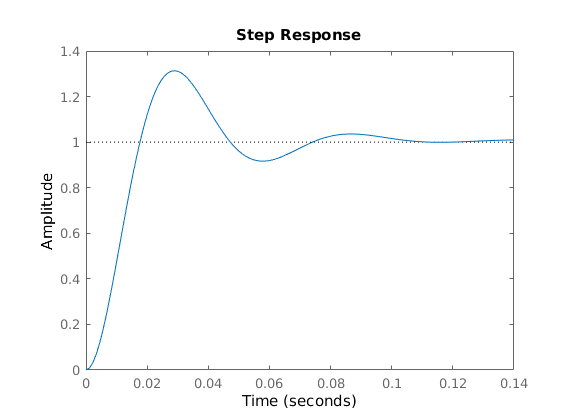
\includegraphics[width=1\linewidth]{image/step_pid_ex_d_mod}
		  \caption{Resposta ao degrau do sistema.}
		  \label{fig:pid_step_d_mod}
		\end{subfigure}%
		\begin{subfigure}{.5\textwidth}
		  \centering
		  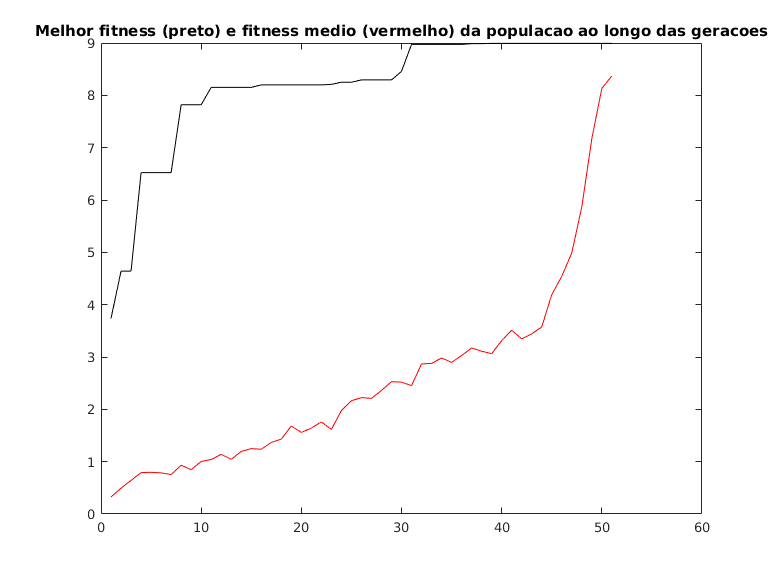
\includegraphics[width=1\linewidth]{image/melhor_fitness_pid_ex_d_mod}
		  \caption{Evolução dos valores da função \textit{fitness}.}
		  \label{fig:pid_fitness_d_mod}
		\end{subfigure}%
		
		\begin{subfigure}{.5\textwidth}
		  \centering
		  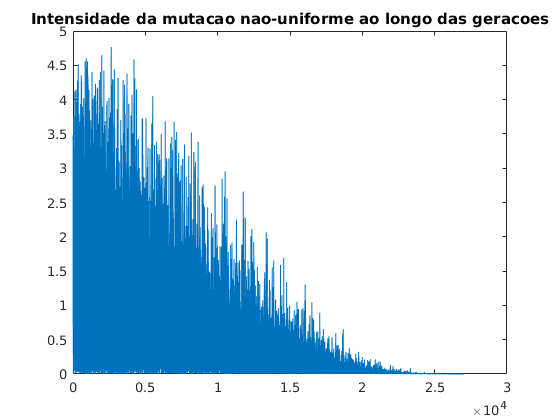
\includegraphics[width=1\linewidth]{image/mutacao_pid_ex_d_mod}
		  \caption{\centering Evolução da intensidade de mutações ao longo das
		  gerações.}
		  \label{fig:pid_mutacao_d_5}
		\end{subfigure}%
		\begin{subfigure}{.5\textwidth}
		  \centering
		  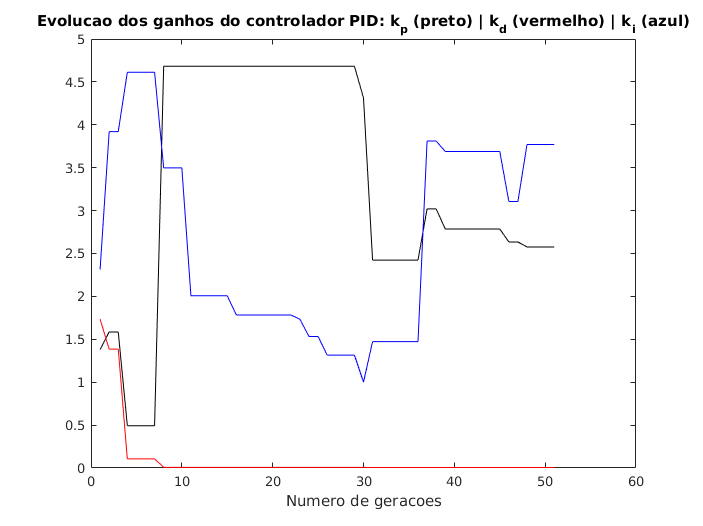
\includegraphics[width=1\linewidth]{image/kp_kd_ki_pid_ex_d_mod}
		  \caption{\centering Evolução dos parâmetros.}
		  \label{fig:pid_parametros_d_mod} 
		\end{subfigure}
	
	\caption{Resultado para a melhor execução do algoritmo evolutivo com
	\textit{fitness} considerando a margem de fase e parâmetros modificados.}
	\end{figure}
	
	\FloatBarrier
	
	Neste caso, como os resultados de cada execução variam bastante, aumentar a
	população e as taxas de \textit{crossover} e mutação contribuem para a obtenção
	de uma solução de melhor qualidade, visto que a diversidade nos indivíduos é
	maior. Logo, a probabilidade que a solução ótima esteja presente em um dos
	indivíduos é consequentemente maior. Uma taxa de mutação elevada também garante
	que mais soluções sejam testadas, à medida que bons indivíduos podem dar origem
	a indivíduos melhores que eles mesmos através da mutação. Enfim, assim como no
	caso em que os parâmetros não tinham sido alterados, a figura
	\ref{fig:pid_fitness_d_mod} revela que a média dos valores de \textit{fitness}
	é muito distante do maior, indicando que nas gerações mais jovens há muitos
	indivíduos ruins. A figura \ref{fig:pid_parametros_d_mod} mostra, por sua vez,
	que, para populações maiores, todos os parâmetros podem variar fortemente
	ao passar das gerações, ao contrário que é observado no caso em que tamanho da
	população é igual a 100. Este fato também é totalmente esperado, visto que,
	para populações maiores, a chance de um indivíduo encontrar um outro melhor que ele
	é maior.
	
\end{enumerate}
